\documentclass[aspectratio=169,10pt]{beamer}
\usetheme{default}
\usecolortheme{seagull}
\setbeamertemplate{navigation symbols}{}
\setbeamertemplate{footline}[frame number]
\setbeamerfont{frametitle}{size=\large,series=\bfseries}
\setbeamercolor{frametitle}{fg=black!85}
\usepackage{graphicx,booktabs}
\graphicspath{{../../figures/}}
\newcommand{\src}[1]{\vfill{\tiny\color{black!55}#1}}
\title{Mapping the Consumption Gap}
\subtitle{Planned Data Center Capacity versus Electricity Supply in California}
\author{Sebastian Oldman\\[3pt]\small M.S. capstone, Computer Science and Engineering, UC Santa Cruz}
\date{Defense deck. Data frozen September 22, 2026}
\begin{document}

\begin{frame}
\titlepage
\end{frame}

\begin{frame}{The question, borrowed from Finland}
\begin{itemize}
\item Finland (Manner, IRTF SUSTAIN, July 2026): about 285~MW of data centers operating, 7,777~MW in the public investment registry.
\item California, December 2025: 23,277~MW of energization requests reported to the CEC, 20,677~MW in the state: 5,086~MW signed, 6,987~MW applications, 8,604~MW inquiries.
\item Existing California data center load: about 1,000~MW, 7.0 to 9.3~TWh a year.
\item The CEC discounts requests with confidence levels, a utilization factor and a ramp. Are the discounts right, can supply keep up, what can flexibility do, and how does the count compare with other regimes?
\end{itemize}
\src{Sources: manner2026; cec\_assembly\_hearing\_2026\_01\_28; cec\_dc\_methodology\_memo\_2026; chapter 1 estimates (ch1\_dc\_load\_estimates.csv).}
\end{frame}

\begin{frame}{Research questions and the method}
\begin{columns}[T]
\column{0.55\textwidth}
\begin{itemize}
\item \textbf{RQ1} Pipeline by stage, absolute and relative to the grid.
\item \textbf{RQ2} The 2030 gap, raw and probability-weighted, in TWh and net-peak MW.
\item \textbf{RQ3} Six counting regimes compared; California's number under each rule.
\item \textbf{RQ4} Headroom from load flexibility as a share of the gap.
\end{itemize}
\column{0.45\textwidth}
\begin{itemize}
\item An independent replication and audit of the CEC method.
\item Every raw file in a manifest (URL, access date, SHA-256); one command per chapter; every figure stamped with its files and manifest ids.
\item Data frozen 2026-09-22; repository tagged; processed outputs exported with the report.
\end{itemize}
\end{columns}
\end{frame}

\begin{frame}{Chapter 1: the grid as it stands}
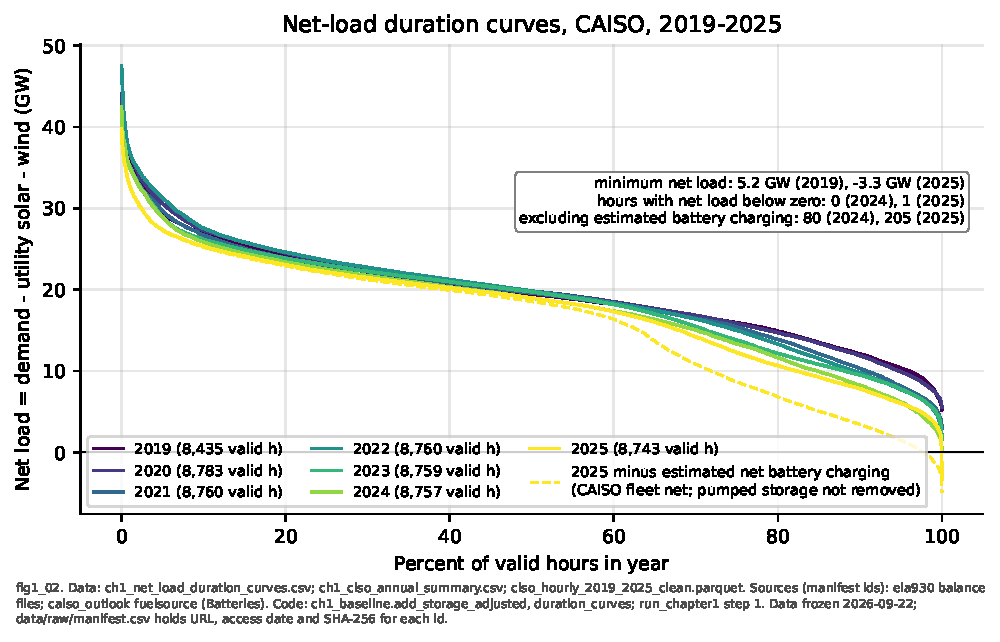
\includegraphics[width=\textwidth,height=0.72\textheight,keepaspectratio]{fig1_02_net_load_duration_curves}
\begin{itemize}\small
\item CAISO demand 2019 to 2025 from EIA-930, cleaned against CAISO's own series; record peak 52,061~MW (2022), 43,860~MW in 2025.
\item Net load after solar and wind now falls below zero for hundreds of hours a year; the evening net peak is what the fleet is planned for.
\end{itemize}
\end{frame}

\begin{frame}{Chapter 1: prices, carbon and existing data center use}
\begin{columns}[T]
\column{0.5\textwidth}
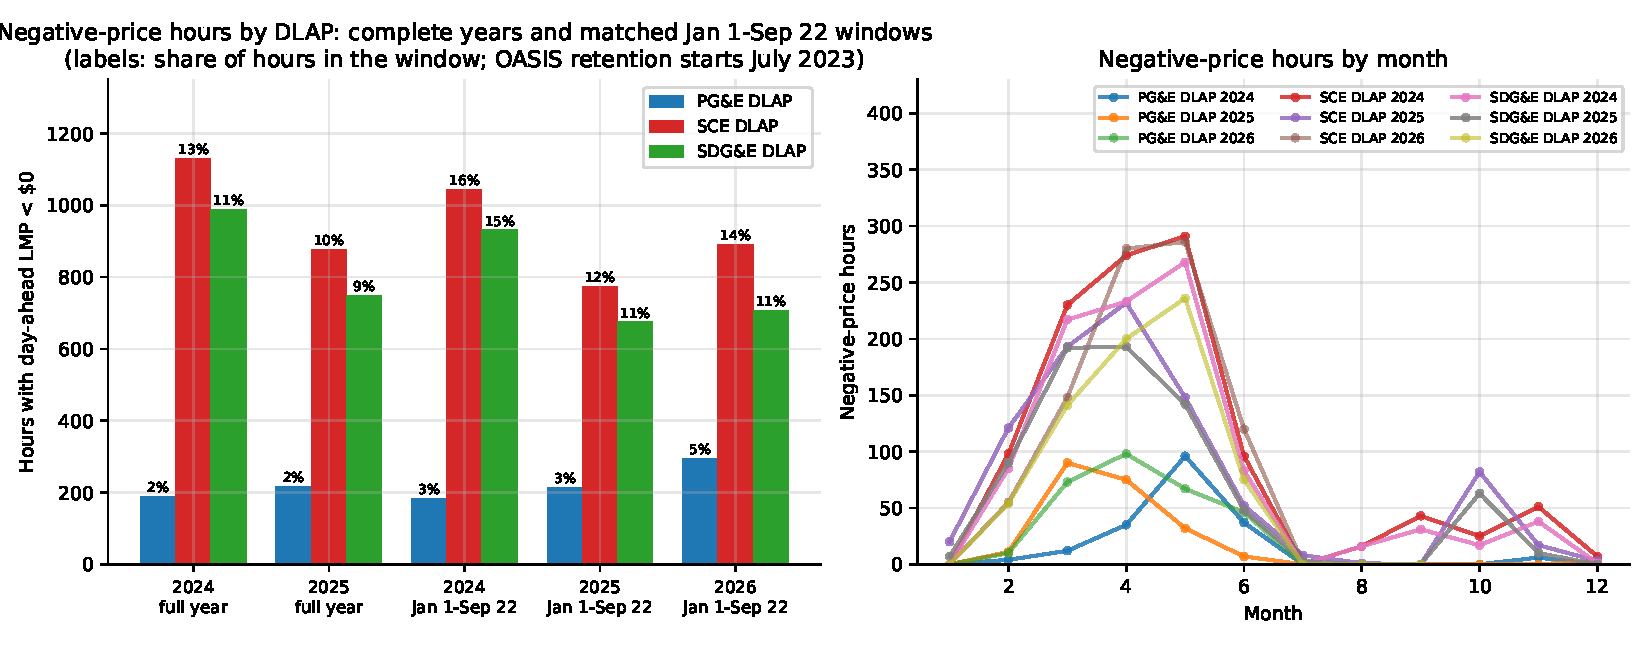
\includegraphics[width=\textwidth]{fig1_06_negative_price_hours}
\column{0.5\textwidth}
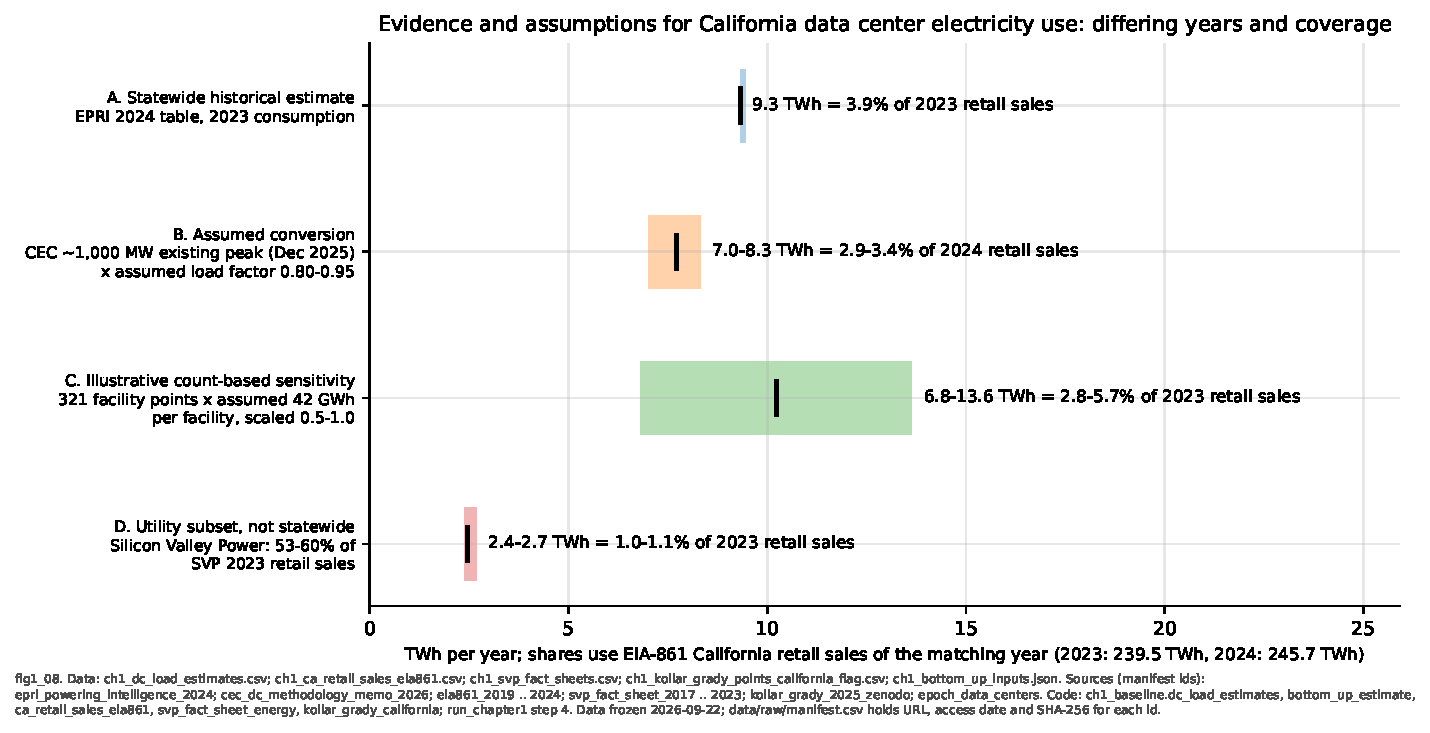
\includegraphics[width=\textwidth]{fig1_08_existing_dc_load_estimates}
\end{columns}
\begin{itemize}\small
\item Negative day-ahead prices in 877 hours at the SCE load-aggregation point in 2025 (1,131 in 2024), 78 percent between 10 and 16 h.
\item Existing data center use, four ways: a statewide estimate, an assumed conversion of the CEC's 1,000~MW, a count-based sensitivity and the Silicon Valley Power cluster. The spread is the finding.
\end{itemize}
\end{frame}

\begin{frame}{Chapter 2: construction broke upward after ChatGPT}
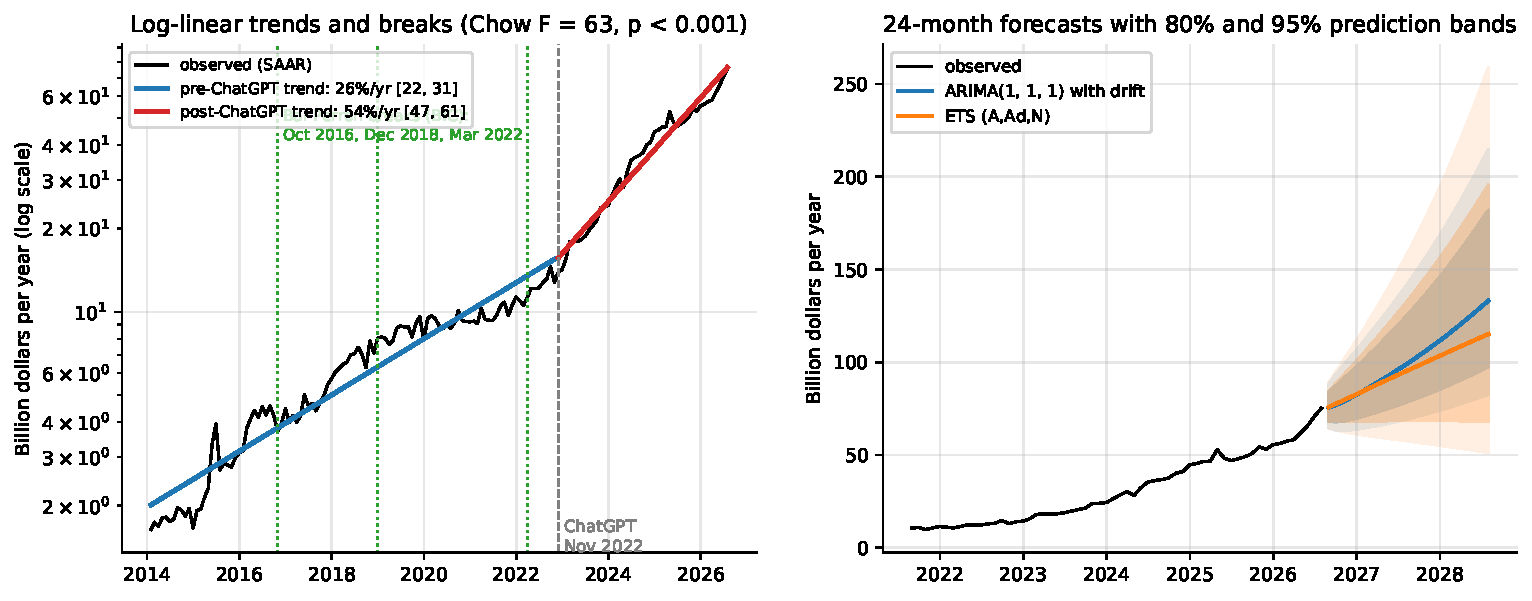
\includegraphics[width=\textwidth,height=0.7\textheight,keepaspectratio]{fig2_02_census_breaks_and_forecast}
\begin{itemize}\small
\item Census data center construction spending: a Chow test at December 2022 and Bai-Perron breaks located by the data agree; ARIMA and ETS bands and a rolling-origin backtest.
\item California has no state construction series; proxies are QCEW employment, CBRE Silicon Valley MW and the Epoch AI hub.
\end{itemize}
\end{frame}

\begin{frame}{RQ1: the pipeline against the grid}
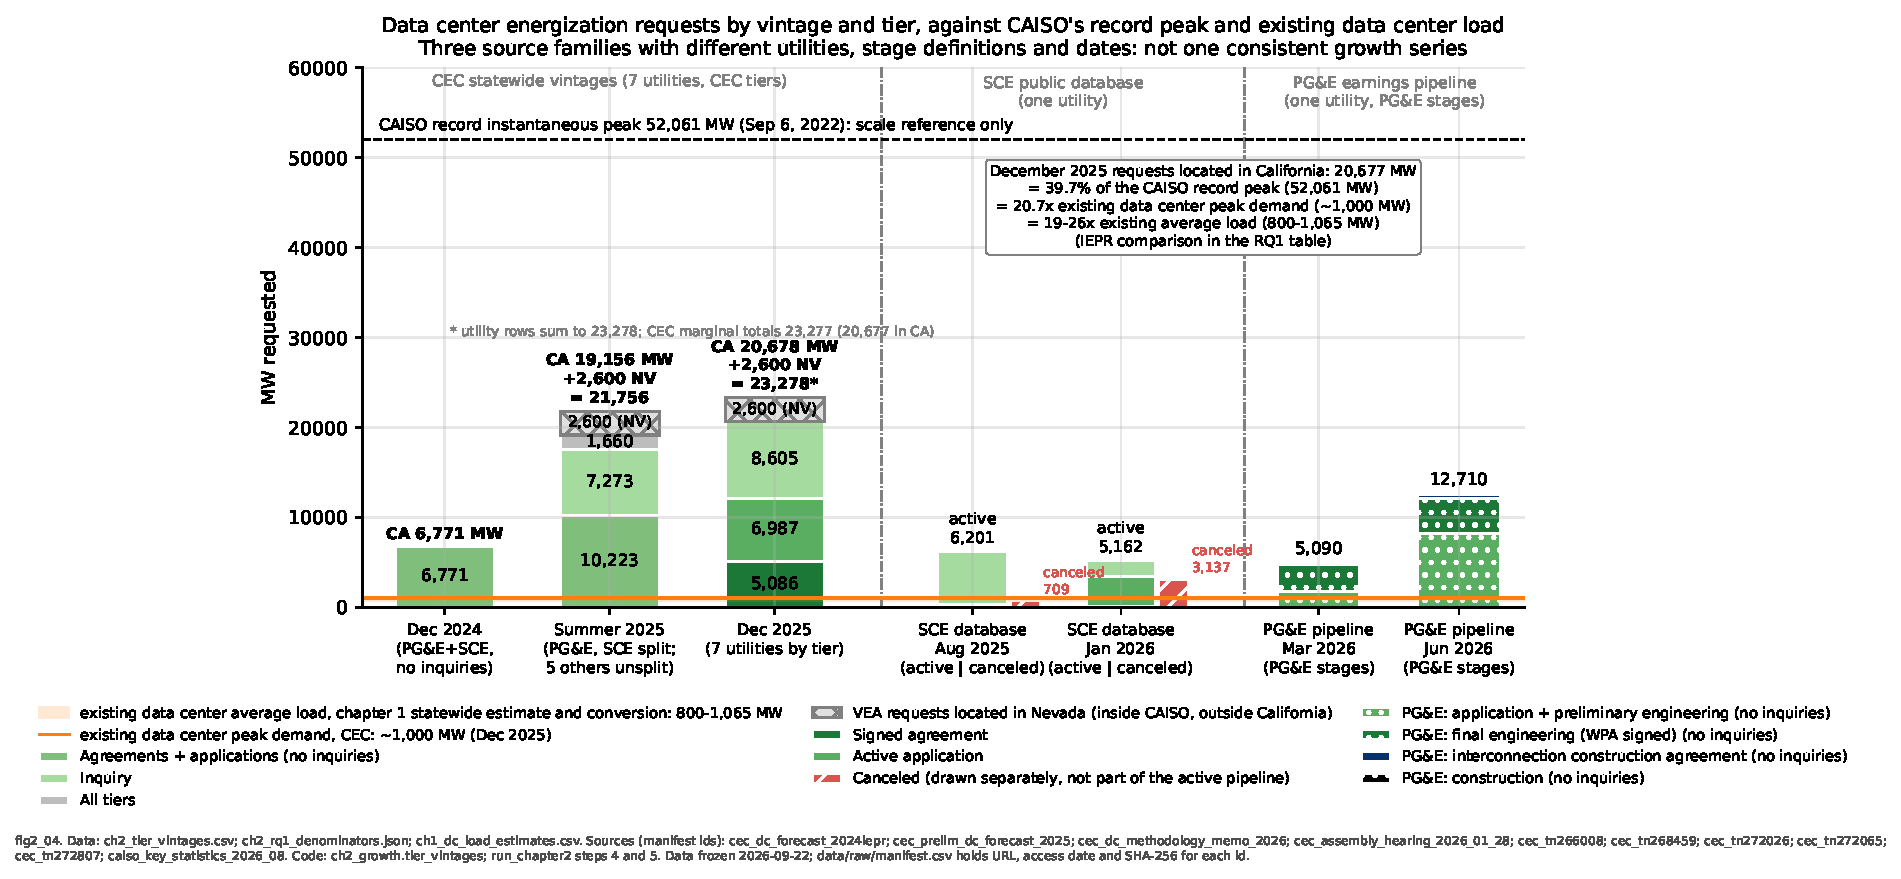
\includegraphics[width=\textwidth,height=0.7\textheight,keepaspectratio]{fig2_04_tier_vintages}
\begin{itemize}\small
\item 20,677~MW in California: 40 percent of the CAISO record peak, twenty times the existing data center peak, five times the IEPR's 2025 to 2030 managed peak growth.
\item VEA's 2,600~MW is in Nevada; SCE's cancellations grew from 709 to 3,137~MW between vintages.
\end{itemize}
\end{frame}

\begin{frame}{Chapter 3: supply history and the fleet}
\begin{columns}[T]
\column{0.5\textwidth}
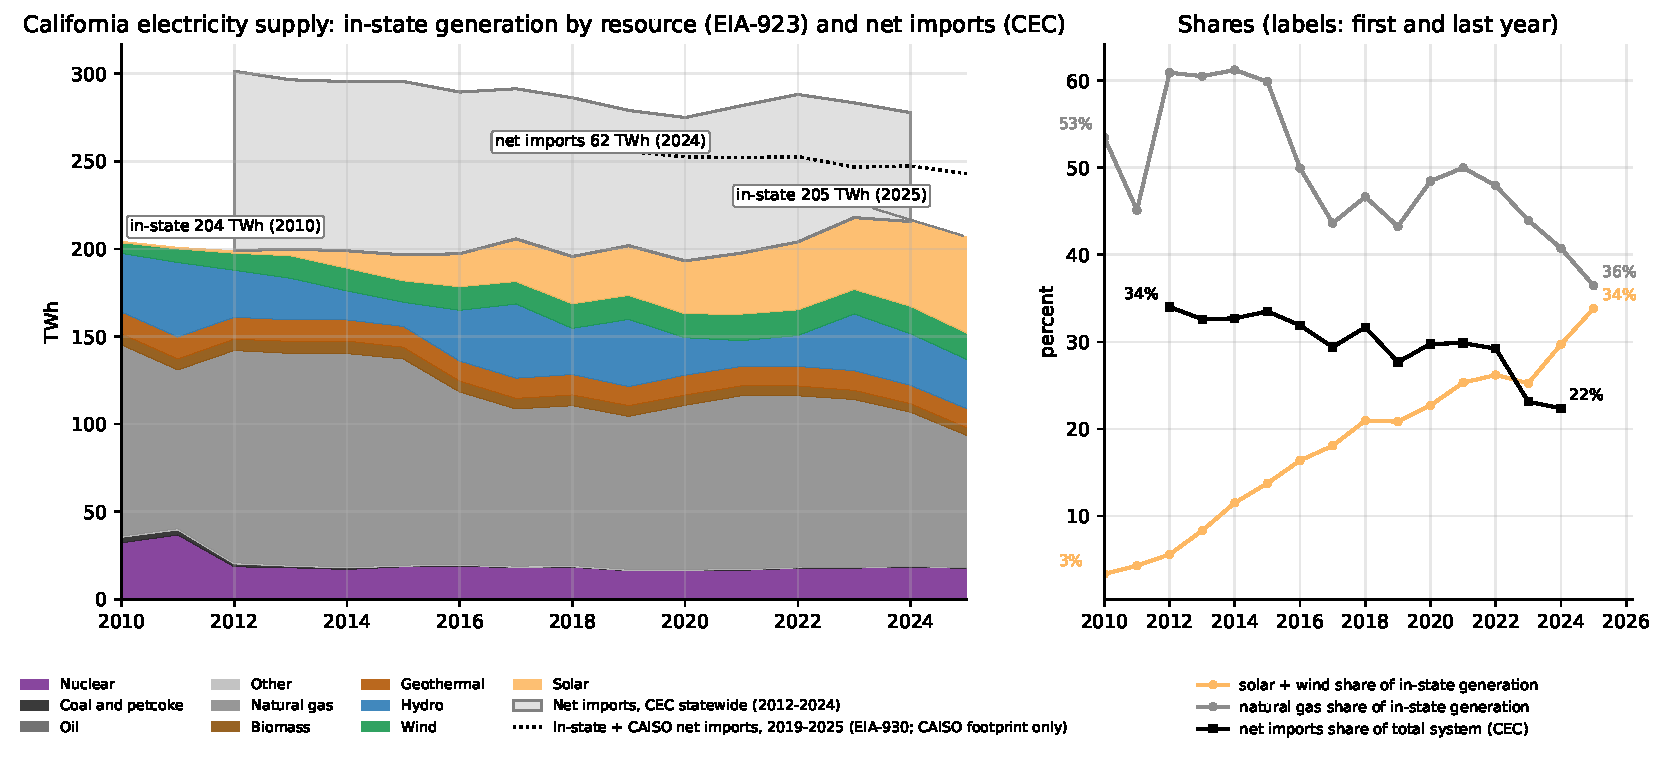
\includegraphics[width=\textwidth]{fig3_01_generation_by_resource}
\column{0.5\textwidth}
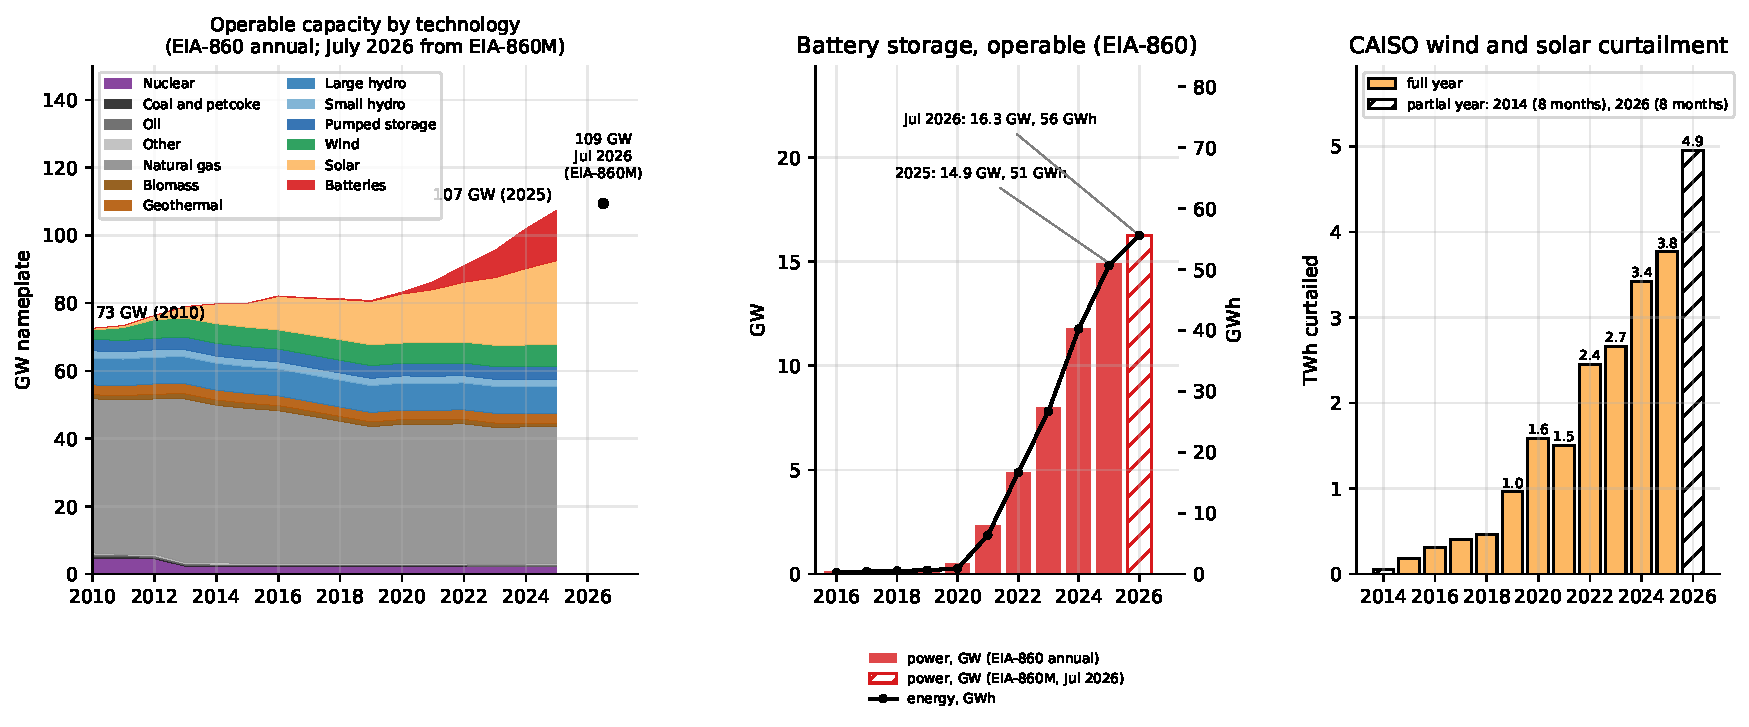
\includegraphics[width=\textwidth]{fig3_02_capacity_storage_curtailment}
\end{columns}
\begin{itemize}\small
\item In-state generation 204~TWh (2010) and 205~TWh (2025); gas 53 to 36 percent, solar and wind 3 to 34 percent; imports 103 to 62~TWh (2012 to 2024).
\item Capacity 73 to 107~GW; batteries 15~GW and 51~GWh; curtailment 3.8~TWh in 2025 and 4.9~TWh in January to August 2026.
\end{itemize}
\end{frame}

\begin{frame}{Chapter 3: what gets built, from California's own record}
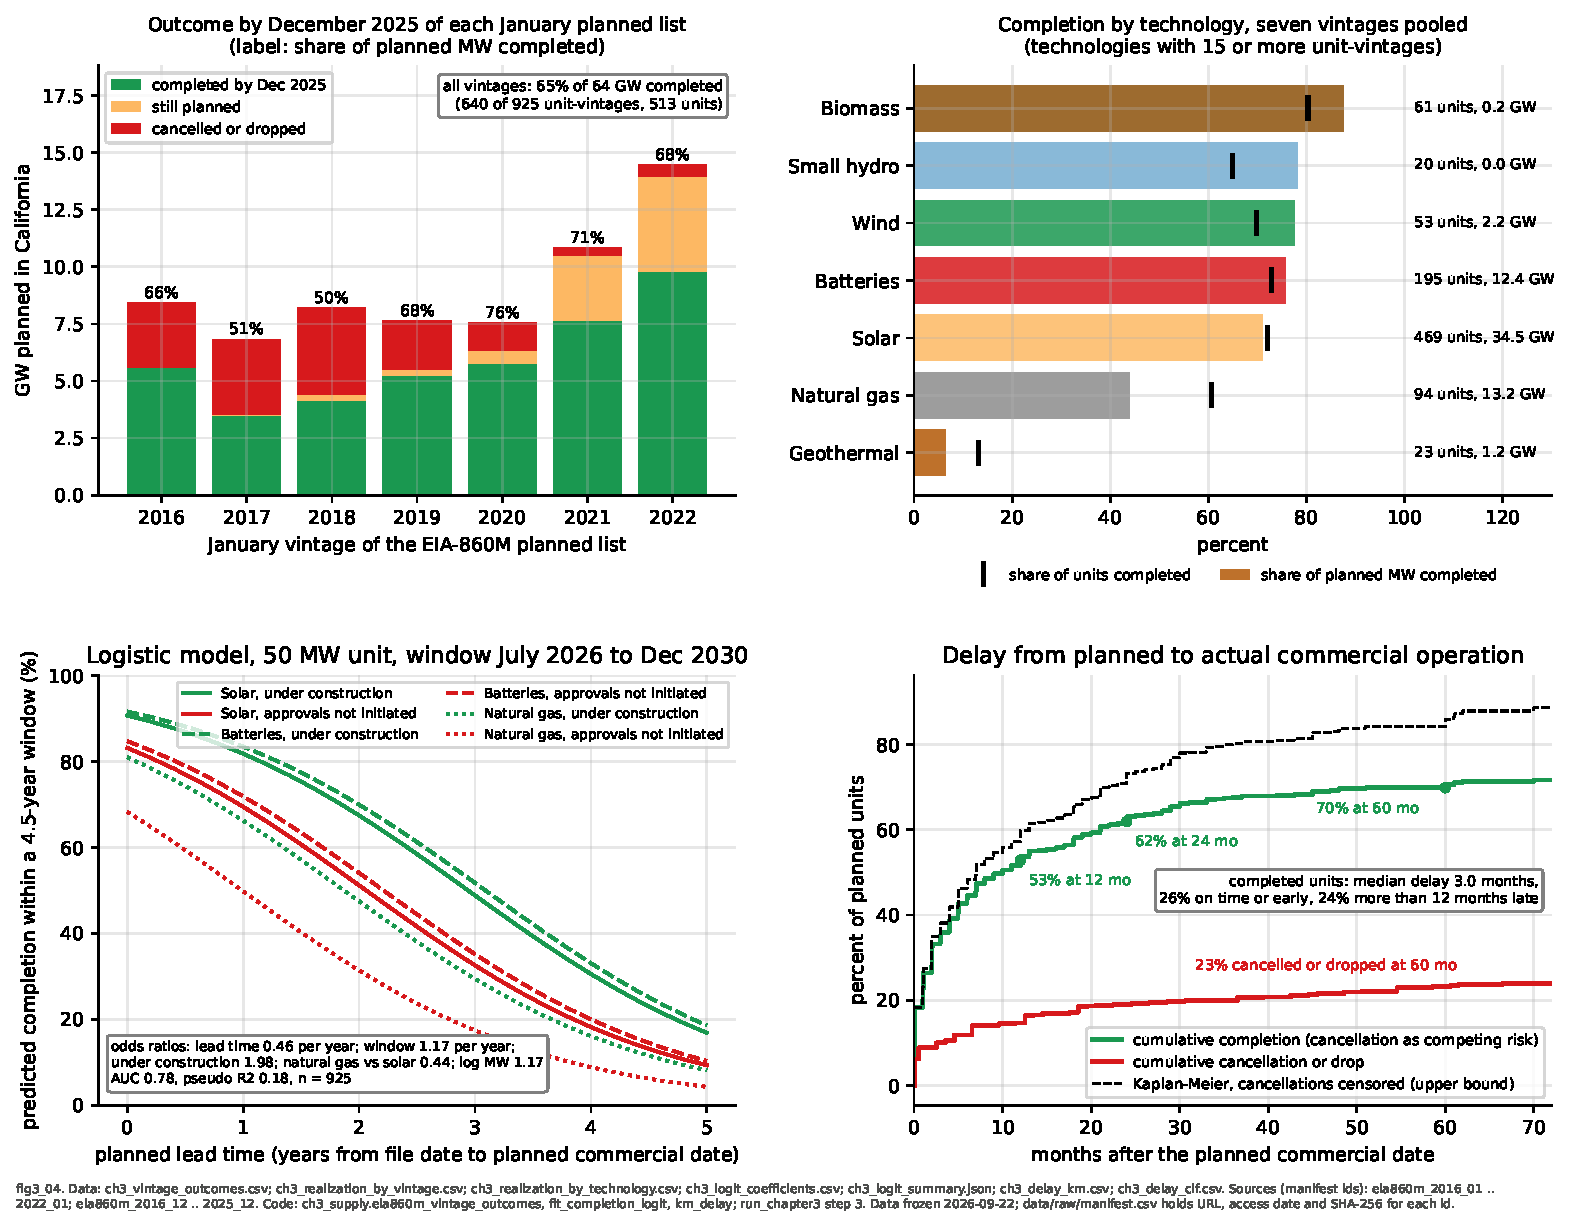
\includegraphics[width=\textwidth,height=0.7\textheight,keepaspectratio]{fig3_04_realization_model}
\begin{itemize}\small
\item 925 unit-vintages of planned generators, January 2016 to 2022, followed to December 2025: 65 percent of megawatts operating; gas 44 percent, geothermal 6 percent.
\item Logistic completion model (lead time, window, status, technology, size) and delay curves with cancellation as a competing risk.
\end{itemize}
\end{frame}

\begin{frame}{Chapter 3: probability-weighted supply in 2030}
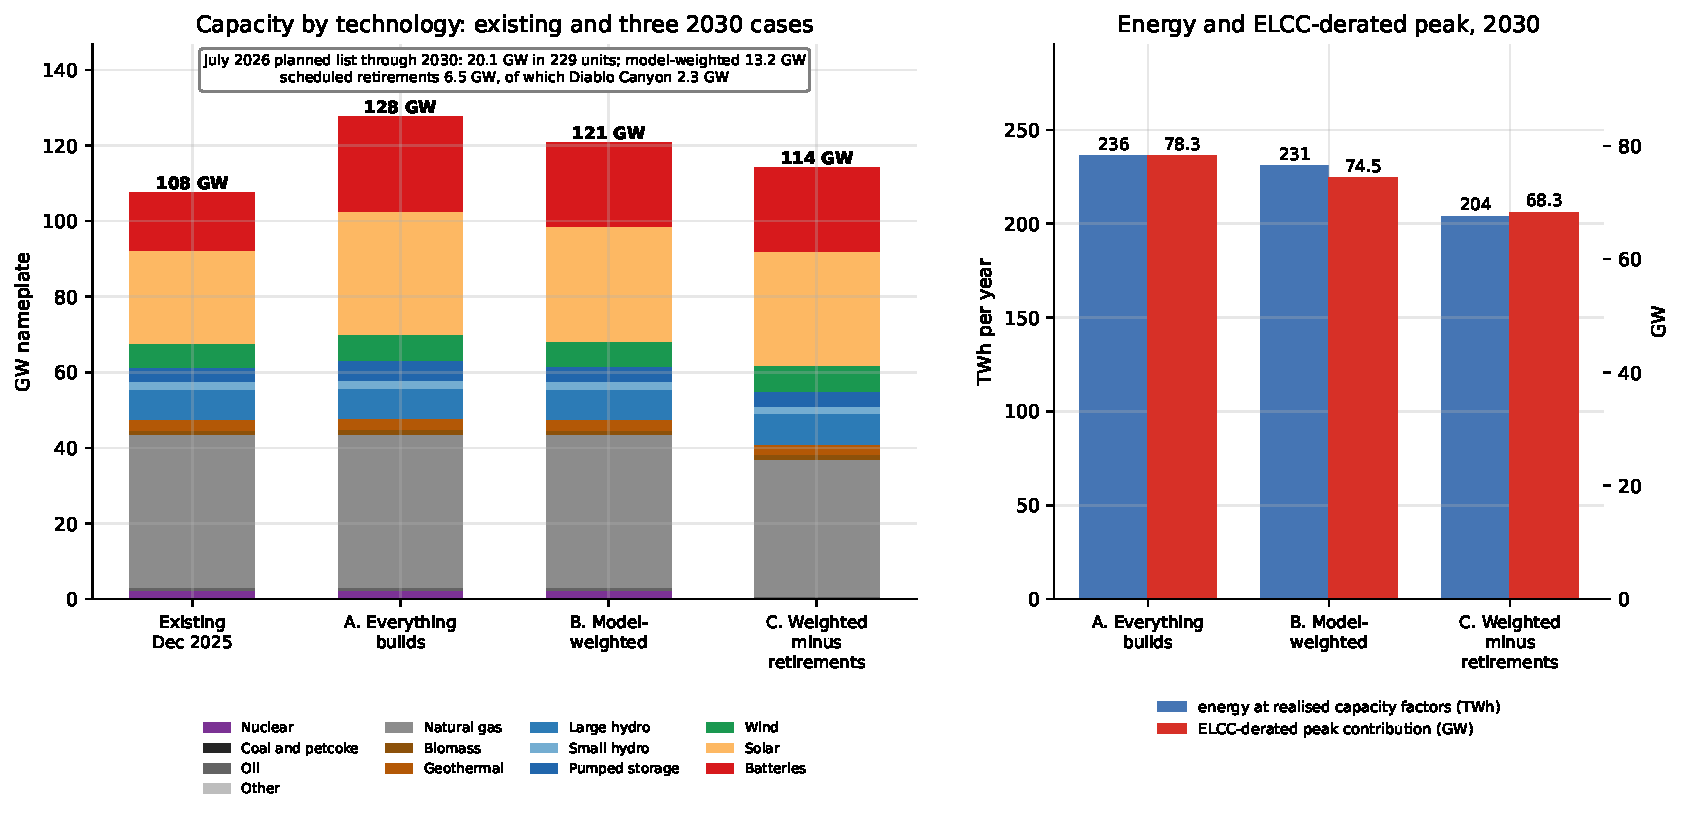
\includegraphics[width=\textwidth,height=0.7\textheight,keepaspectratio]{fig3_05_cases_2030}
\begin{itemize}\small
\item Everything builds: 128~GW, 236~TWh, 78~GW of ELCC. Model-weighted: 121~GW, 231~TWh, 74~GW. Minus 6.5~GW of retirements including Diablo Canyon: 114~GW, 204~TWh, 68~GW.
\end{itemize}
\end{frame}

\begin{frame}{Chapter 4: the same requests under four counting rules}
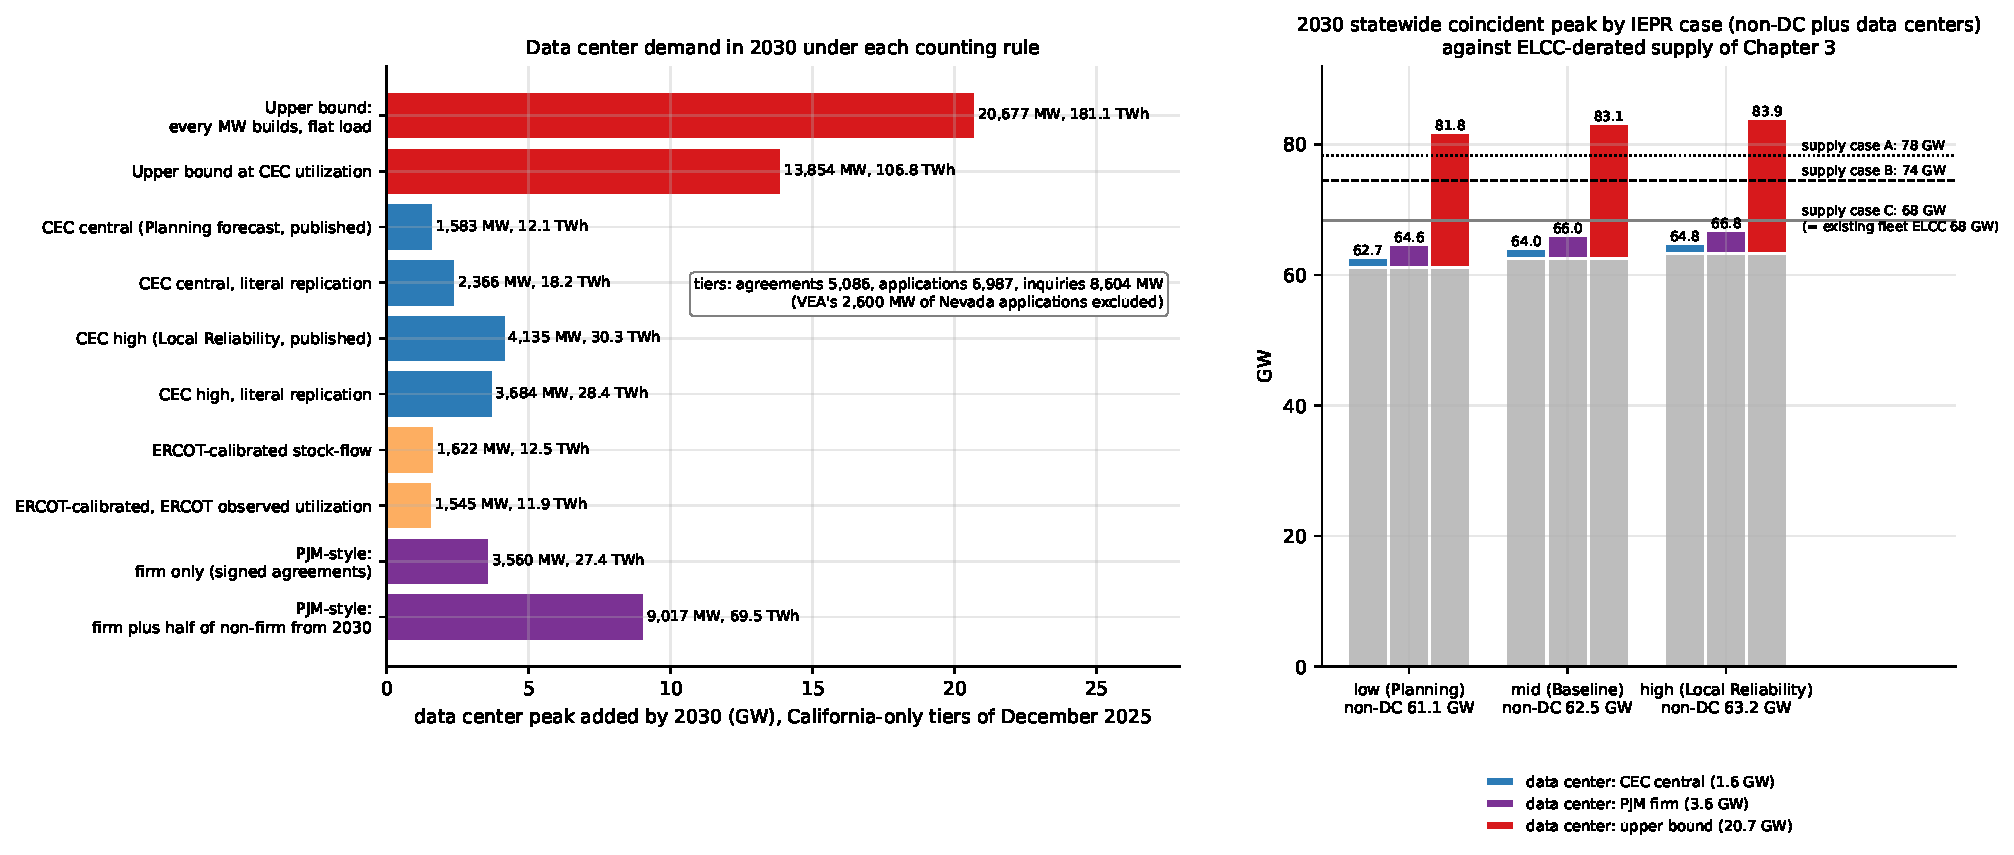
\includegraphics[width=\textwidth,height=0.7\textheight,keepaspectratio]{fig4_01_demand_scenarios_2030}
\begin{itemize}\small
\item Upper bound 20,677~MW and 181~TWh; CEC central 1,583~MW (rebuilt from its parameters: 1,549); CEC high 4,135; ERCOT-calibrated 1,622; PJM firm-only 3,560.
\item The CEC parameters with SVP exempt reproduce its 2040 endpoints (4,855 and 7,381~MW) to within 1~MW.
\end{itemize}
\end{frame}

\begin{frame}{RQ2: the 2030 gap, 10,000 draws}
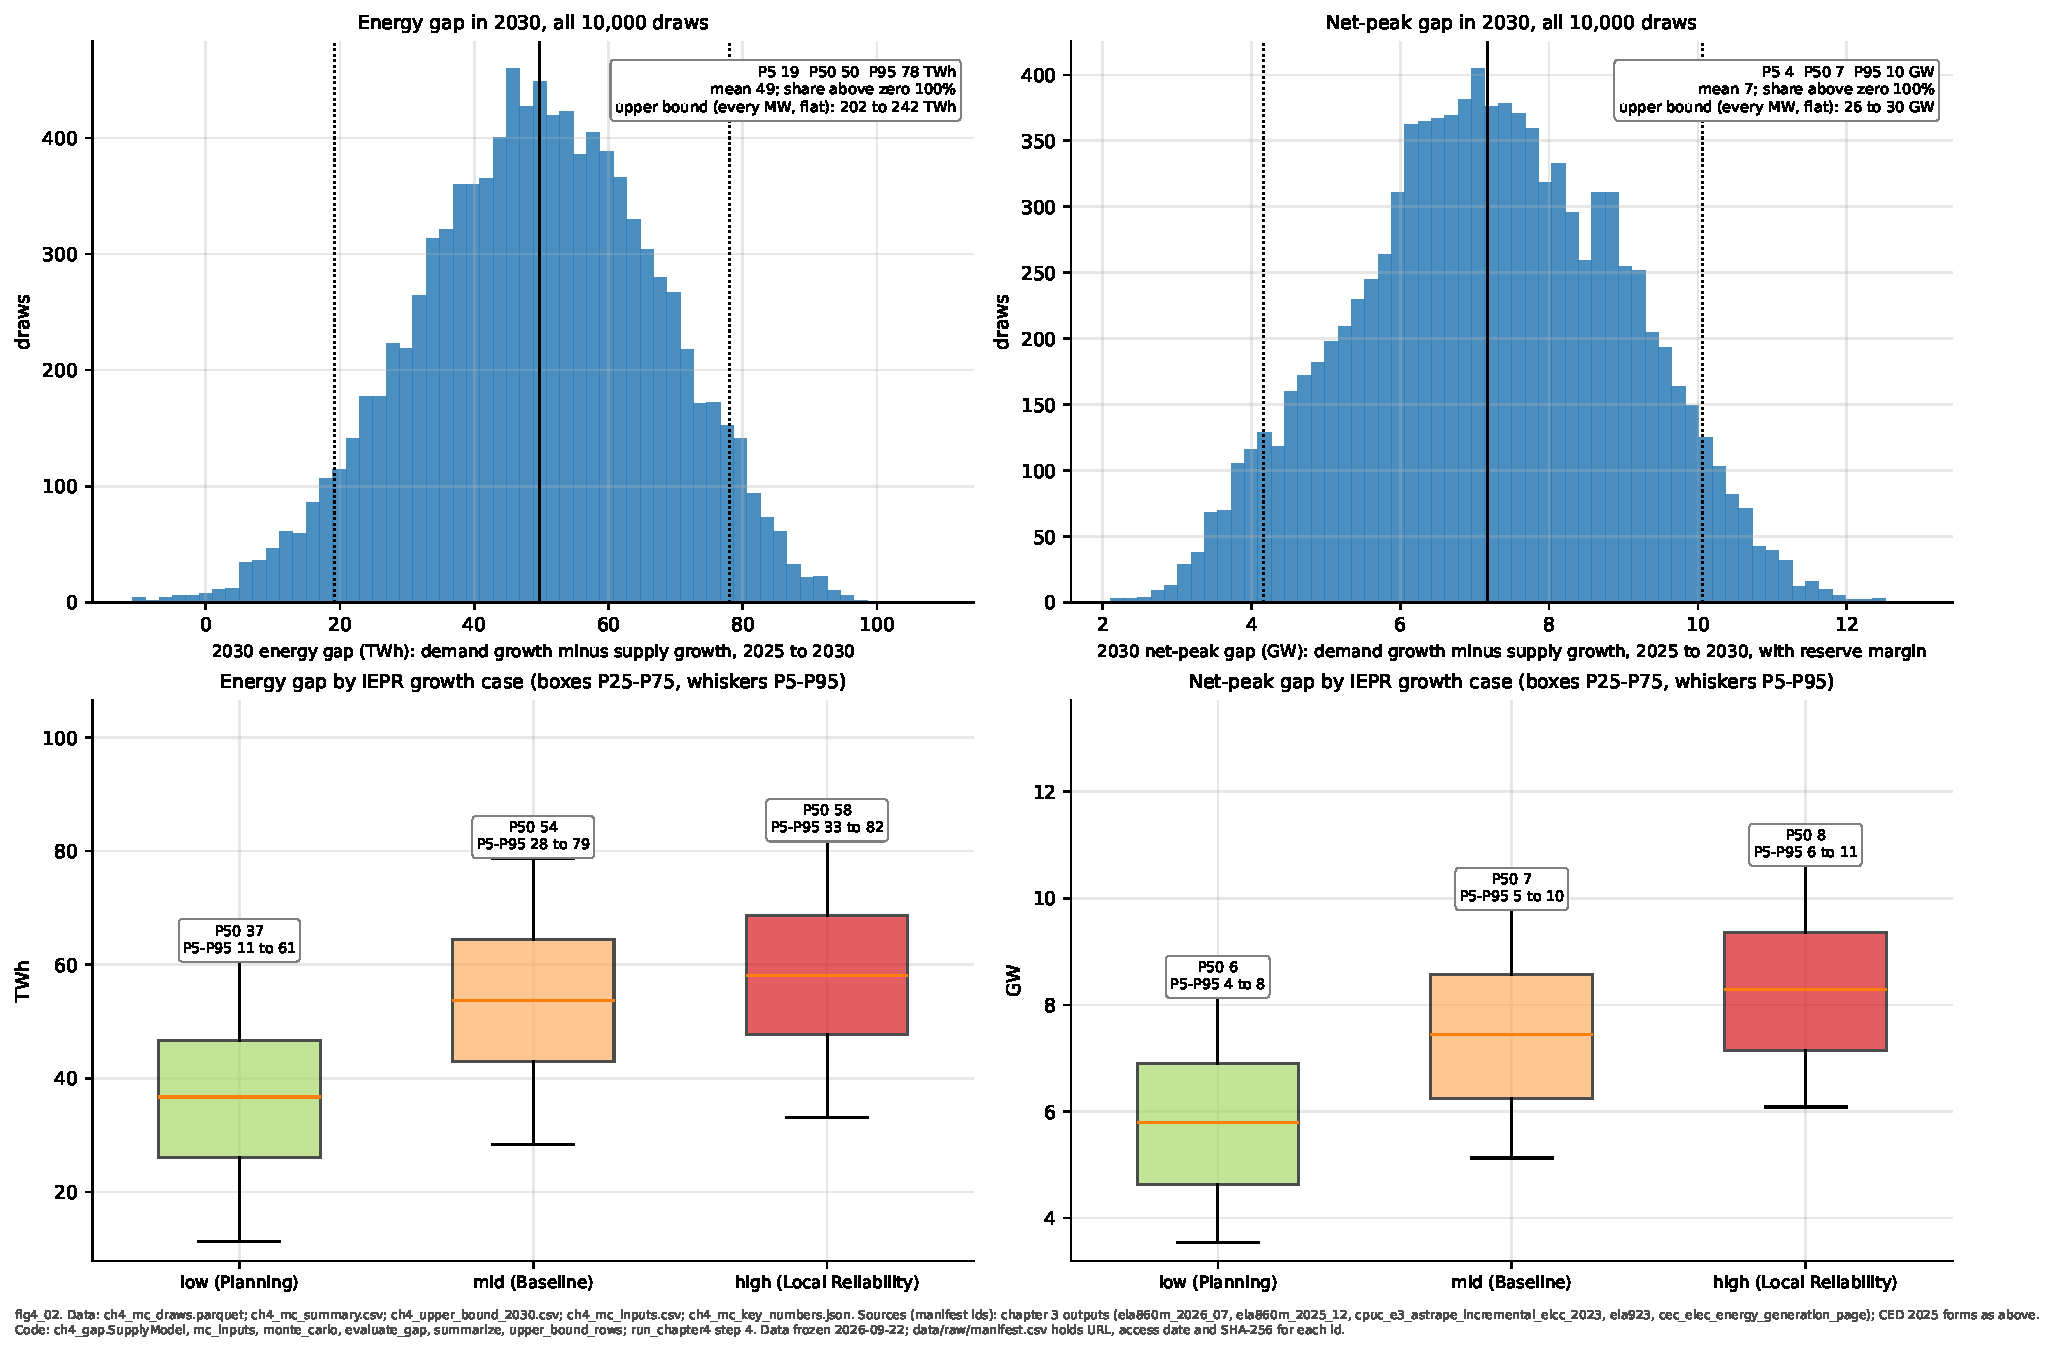
\includegraphics[width=\textwidth,height=0.7\textheight,keepaspectratio]{fig4_02_gap_distributions}
\begin{itemize}\small
\item Energy gap 50~TWh at the median (19 to 78); net-peak gap 7.2~GW (4.2 to 10.1). Data centers: 18~TWh and 2.3~GW of it.
\item Upper bound: 202 to 242~TWh and 25.5 to 30.2~GW, four to five times the weighted 95th percentile. Gas at a 0.40 capacity factor would close the median energy gap.
\end{itemize}
\end{frame}

\begin{frame}{What drives the answer}
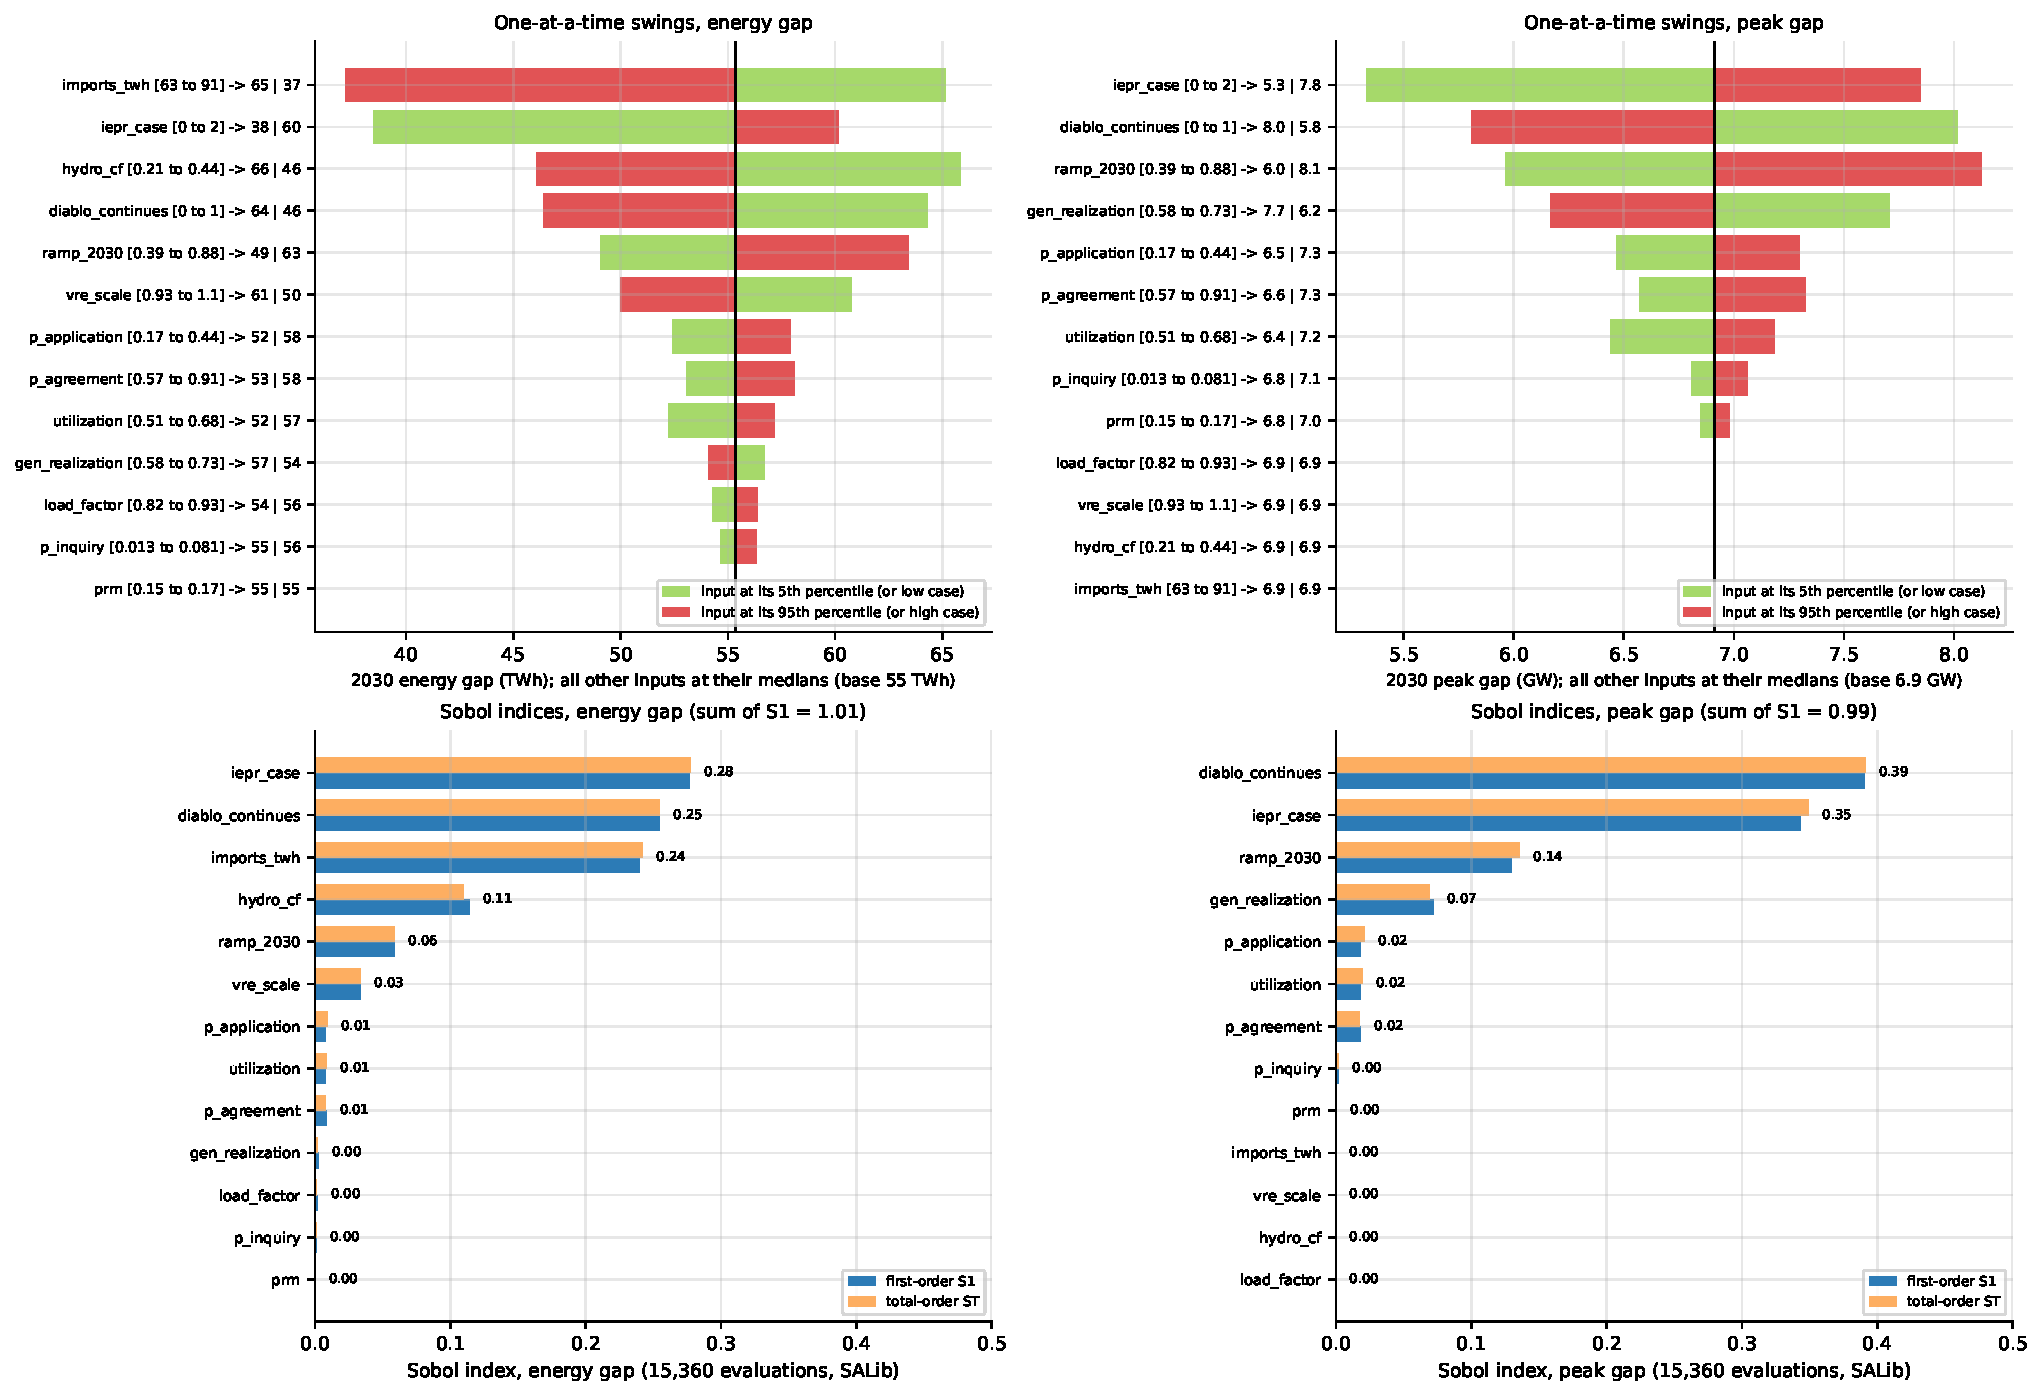
\includegraphics[width=\textwidth,height=0.7\textheight,keepaspectratio]{fig4_03_sensitivity}
\begin{itemize}\small
\item Energy gap: imports, the IEPR case, hydro and Diablo Canyon; the three tier probabilities carry about 2 percent of the energy gap's variance and 4 percent of the peak gap's.
\item Peak gap: Diablo Canyon (total index 0.39), the IEPR case (0.35), the data center ramp (0.14), generation completion (0.07).
\end{itemize}
\end{frame}

\begin{frame}{RQ4: headroom from flexibility}
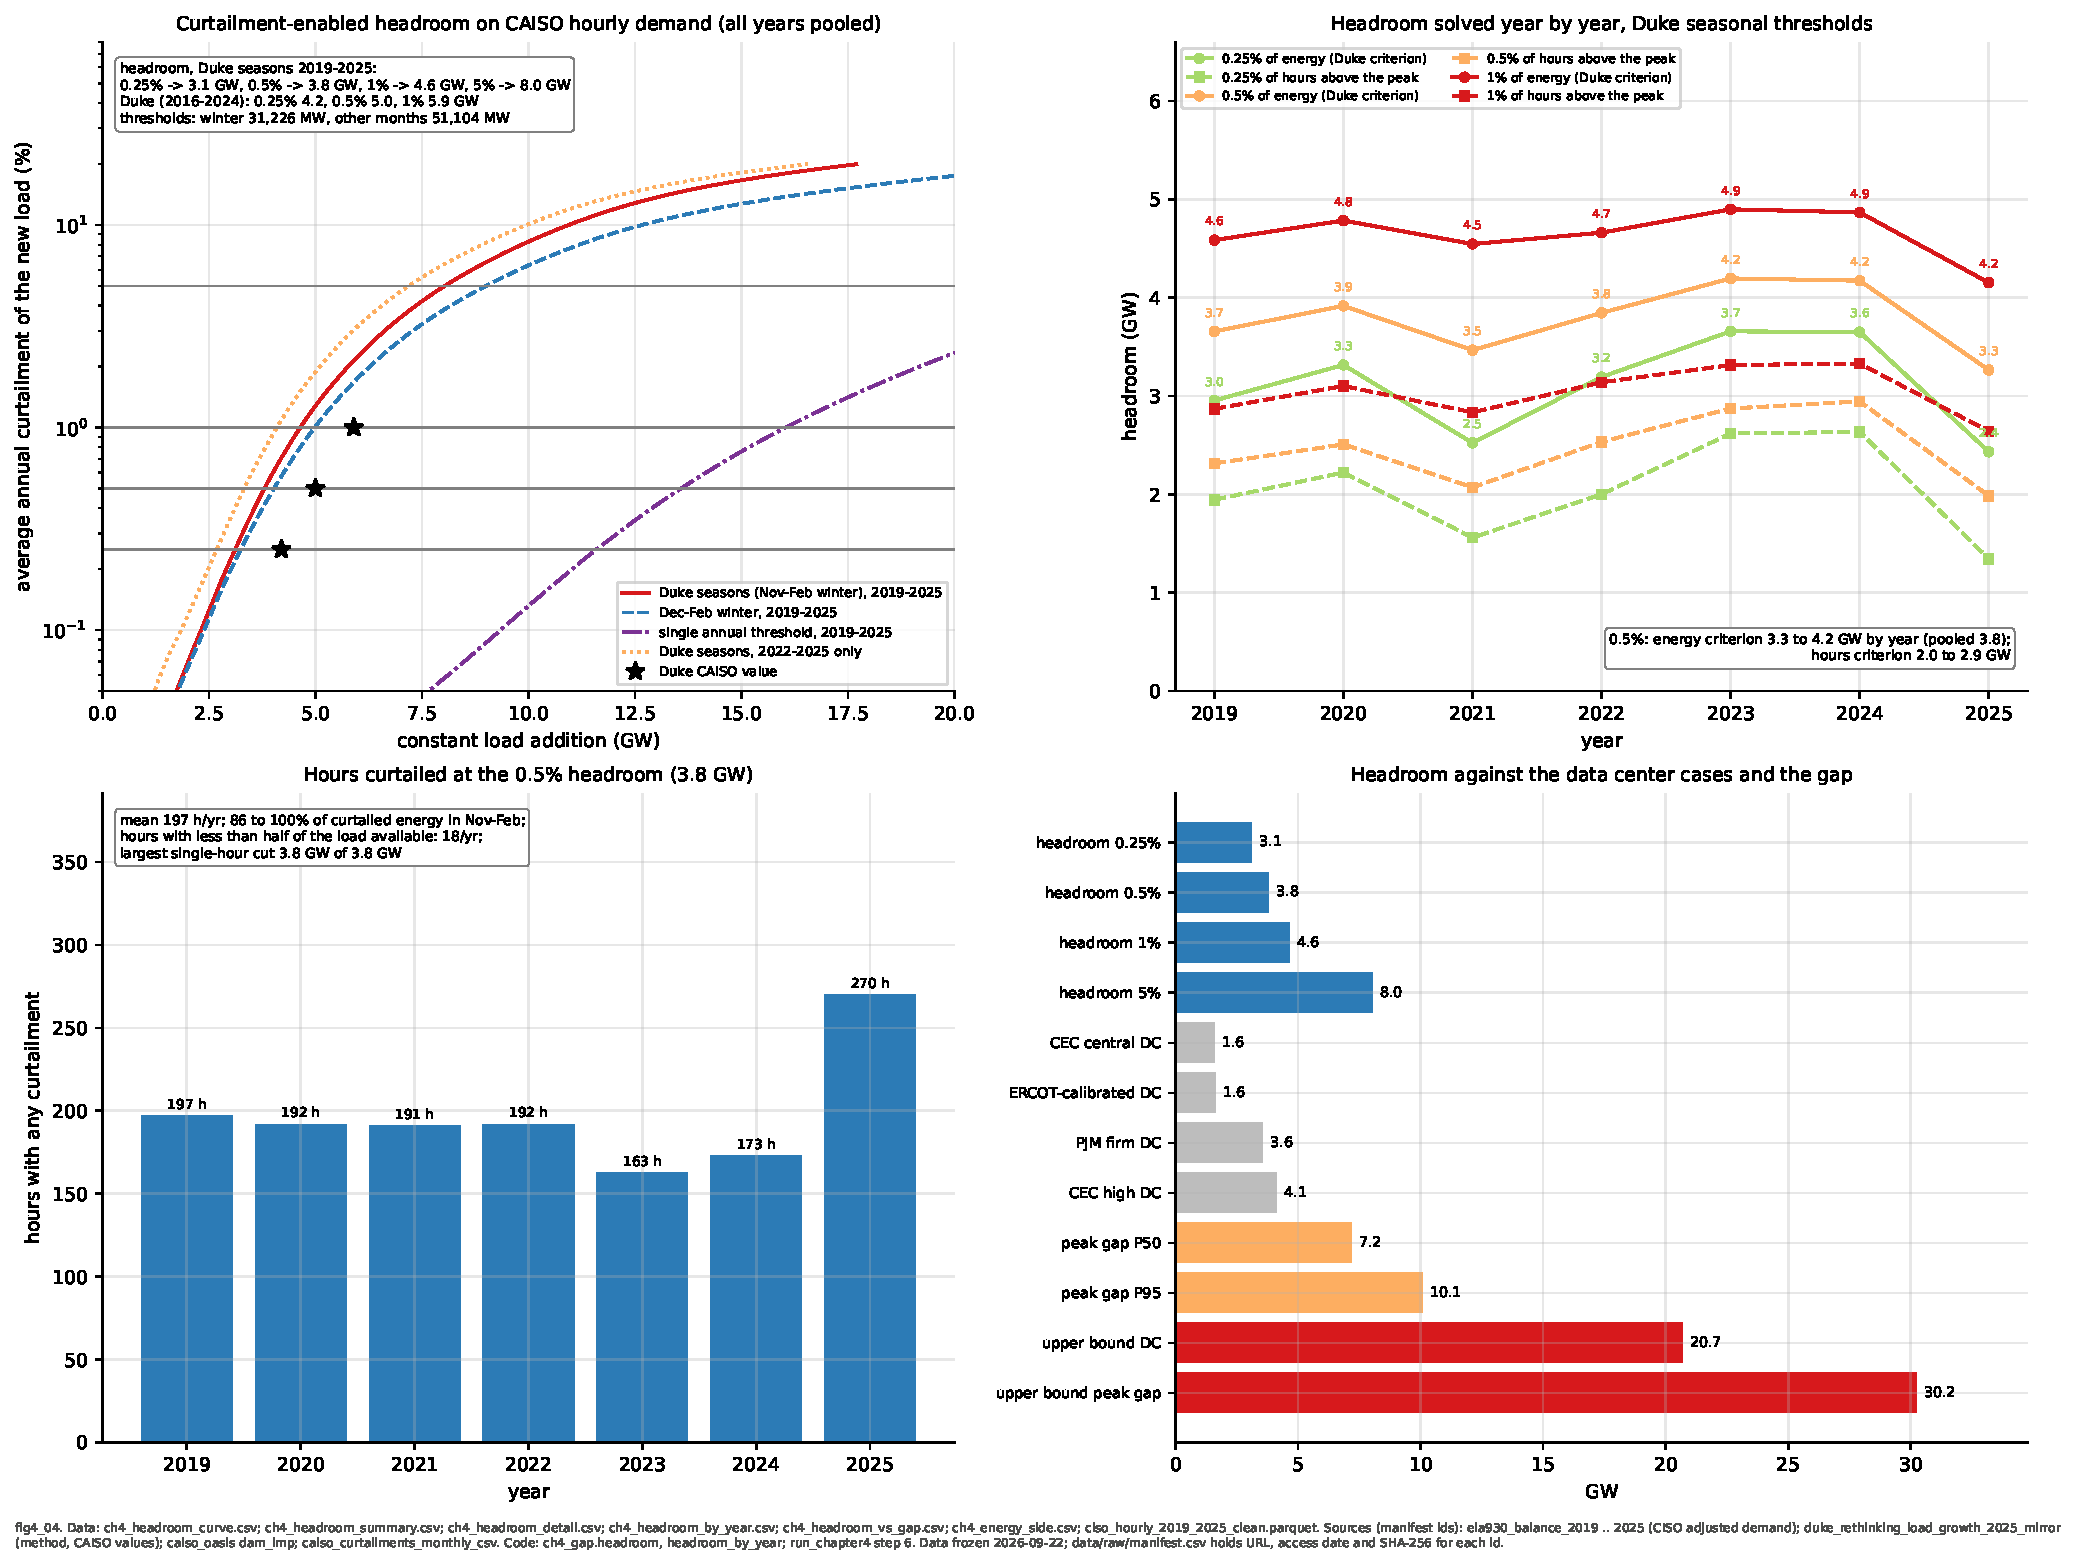
\includegraphics[width=\textwidth,height=0.7\textheight,keepaspectratio]{fig4_04_headroom}
\begin{itemize}\small
\item Duke's method on CAISO load 2019 to 2025: 3.1, 3.8, 4.6 and 8.0~GW at 0.25, 0.5, 1 and 5 percent curtailment (Duke: 4.2, 5.0, 5.9); 98 percent of it in November to February.
\item 3.8~GW is 2.4 times the CEC central data center addition, 53 percent of the median peak gap, 13 percent of the upper-bound gap.
\end{itemize}
\end{frame}

\begin{frame}{RQ3: the ERCOT queue as evidence, and six regimes scored}
\begin{columns}[T]
\column{0.58\textwidth}
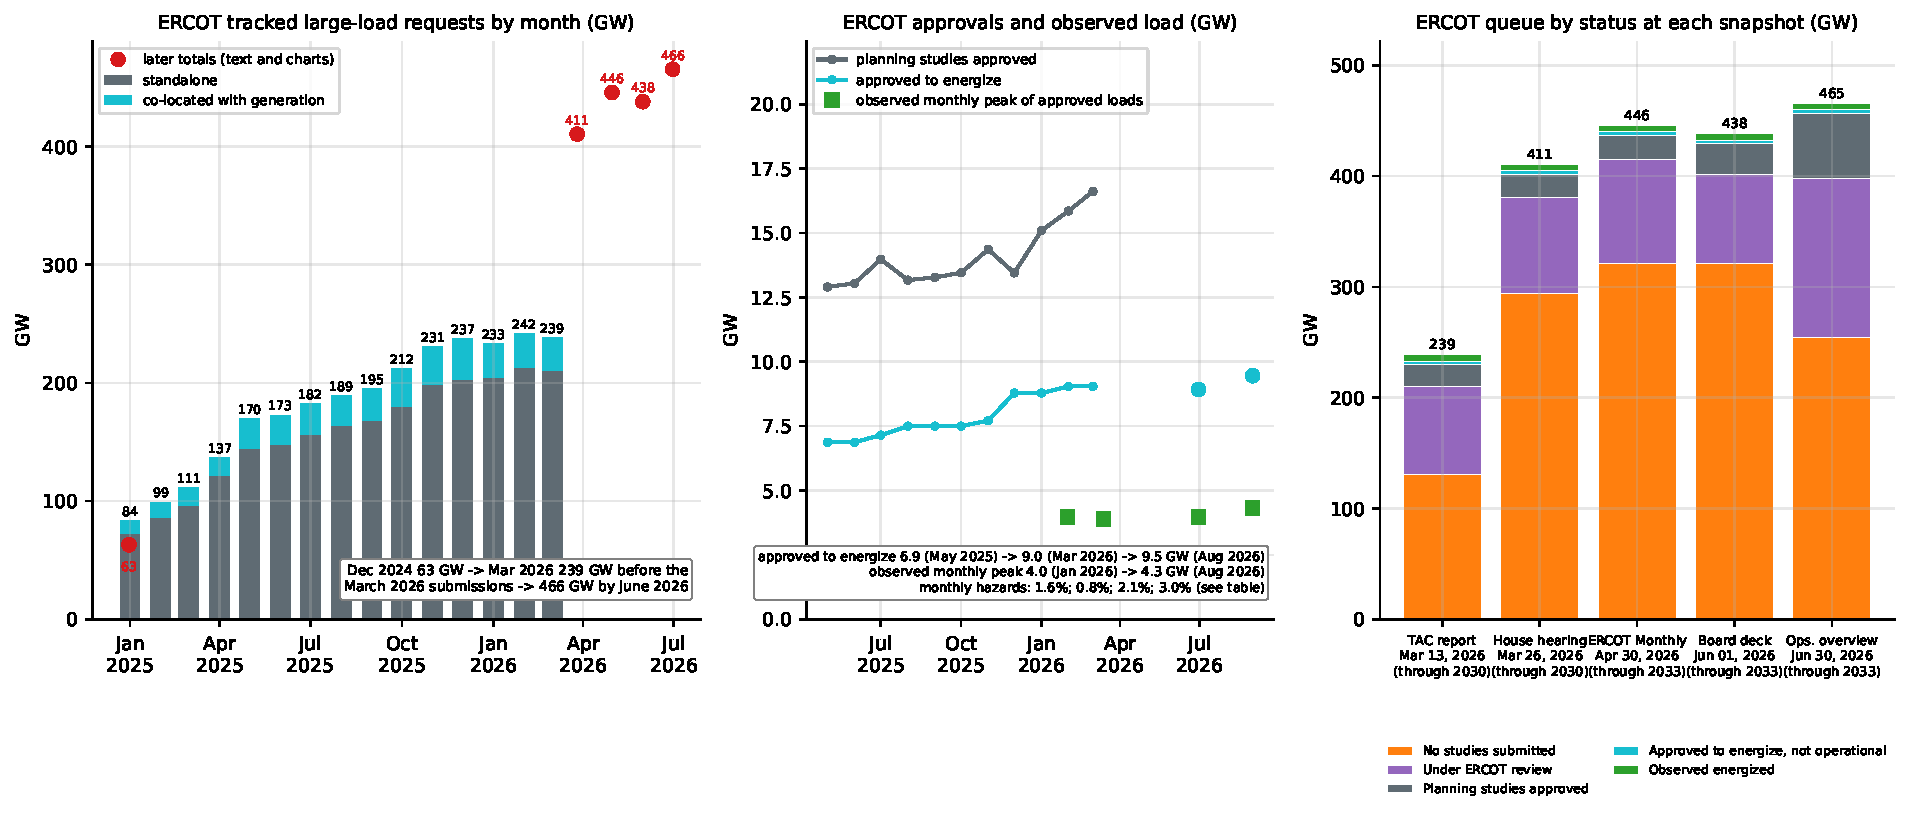
\includegraphics[width=\textwidth]{fig4_05_ercot_queue}
\column{0.42\textwidth}
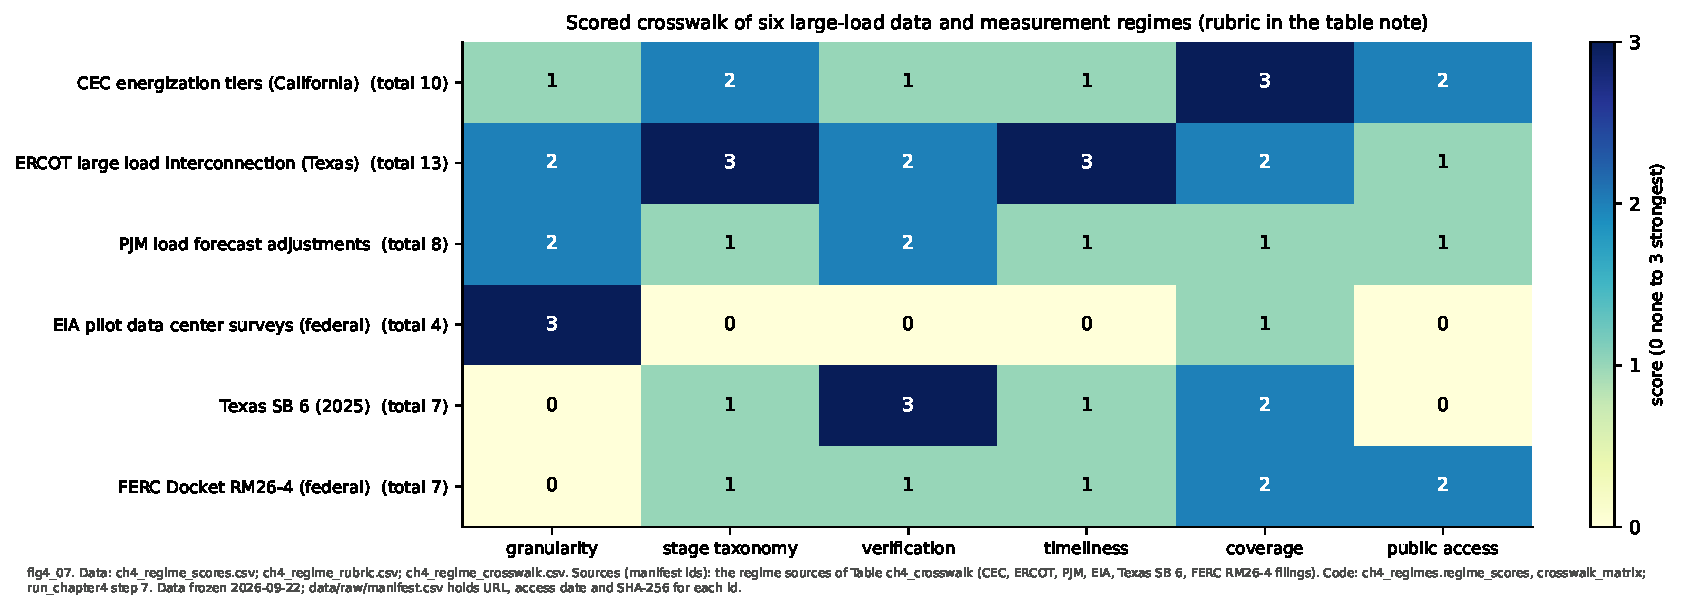
\includegraphics[width=\textwidth]{fig4_07_regime_scores}
\end{columns}
\begin{itemize}\small
\item ERCOT: 63~GW (Dec 2024) to 467~GW (Jul 2026) of requests; approvals to energize 6.9 to 9.5~GW; observed load near 4~GW.
\item Scores of 18: ERCOT 13, CEC 10, PJM 8, Texas SB 6 and FERC RM26-4 7, EIA pilot 4. Same requests: 20,677~MW (CEC, ERCOT rules), 5,086 (PJM, Texas forecast rule), about 2,400 (ERCOT rates), about 1,000 (measured).
\end{itemize}
\end{frame}

\begin{frame}{Flexibility also cuts emissions}
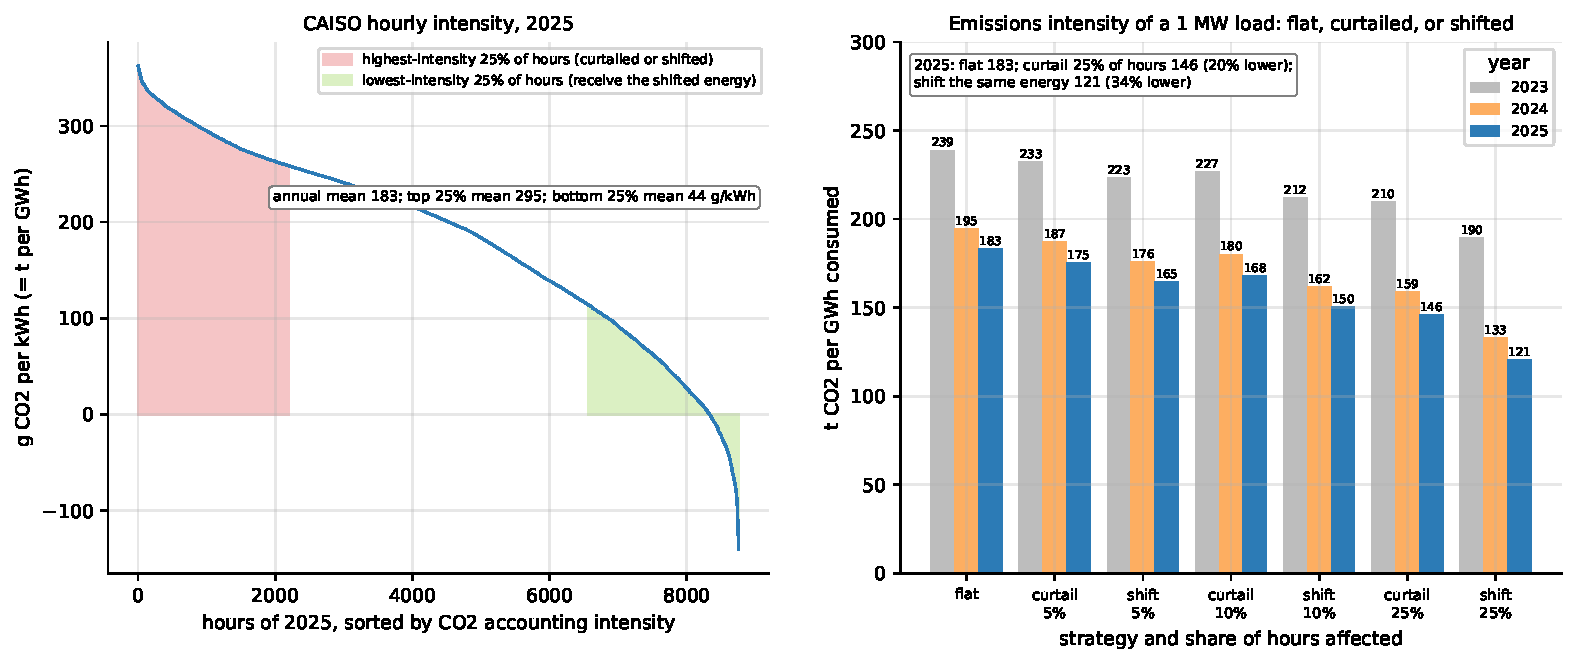
\includegraphics[width=\textwidth,height=0.7\textheight,keepaspectratio]{fig4_06_emissions_flat_vs_flexible}
\begin{itemize}\small
\item A flat load carried 183~t of CO$_2$ per GWh in 2025; curtailing the highest-intensity quarter of hours cuts that by 20 percent, shifting the energy into the lowest-intensity quarter by 34 percent.
\end{itemize}
\end{frame}

\begin{frame}{Contribution: a replication and audit, not a new forecast}
\begin{itemize}
\item The CEC's published parameters rebuild its forecast: exact at the 2040 endpoints, within 2 to 6 percent in 2030 once the SVP exemption is applied.
\item The supply side is discounted with the same discipline, from California's own completion record.
\item The confidence levels are tested against ERCOT's realized transition rates and PJM's firm rule; the gap is a distribution with a stated upper bound and named drivers.
\item Headroom replicated on CAISO load and expressed as a share of the gap; six regimes scored on one rubric.
\item Everything reproducible: manifest, one command per chapter, stamped figures, frozen data, tagged repository, exported outputs.
\end{itemize}
\end{frame}

\begin{frame}{Policy implications}
\begin{itemize}
\item \textbf{CEC:} publish requests at project level with size, requested year and status history (as SCE does); report monthly by phase (as ERCOT does); publish firm and non-firm components separately (as PJM does); state the SVP exemption and the Nevada request where totals appear.
\item \textbf{CPUC and CAISO:} a flexible interconnection service is worth 3 to 5~GW of headroom, mostly winter evenings, plus the midday surplus energy; FERC's June 2026 orders ask for exactly that.
\item \textbf{Resource planning:} weight planned generation by completion probability, updated yearly from EIA-860M.
\item \textbf{Legislature:} Diablo Canyon moves the gap more than any data center assumption (18~TWh, 2.2~GW); licences are in hand, state law stops at 2030.
\item \textbf{EIA:} extend the pilot survey to California.
\end{itemize}
\end{frame}

\begin{frame}{Limits}
\begin{itemize}
\item Boundaries: CAISO hourly data against statewide generation and forecast; imports' peak contribution outside the absolute balance.
\item ERCOT hazards measured during a surge; several ERCOT and PJM values read from chart images.
\item ELCC from the CPUC's 2023 study; reserve margin an assumed range; Diablo Canyon a coin flip with the licence facts stated.
\item Data center load flat at the peak; 2030 energy annualized at the end-2030 level.
\item No project-level California request data outside SCE; the CEC's utility ramp schedules are not public.
\end{itemize}
\end{frame}

\begin{frame}{Conclusion}
\begin{itemize}
\item \textbf{RQ1} 20,677~MW in three tiers: 40 percent of the record peak, twenty times existing data center load.
\item \textbf{RQ2} 2030 gap 50~TWh and 7.2~GW at the median (data centers 18~TWh, 2.3~GW); upper bound 202 to 242~TWh, 25 to 30~GW.
\item \textbf{RQ3} Same requests: 20,677 / 5,086 / about 2,400 / about 1,000~MW under the four counting rules; regimes differ most in timeliness, verification and access.
\item \textbf{RQ4} 3.8~GW of headroom at 0.5 percent curtailment: twice the weighted data center load, half the weighted peak gap, under a fifth of the upper bound.
\item The method is the result: a forecast anyone can rebuild, a supply side discounted the same way, a gap with its uncertainty and drivers named.
\end{itemize}
\end{frame}

\begin{frame}{Backup: reproducibility}
\begin{itemize}\small
\item Repository: \texttt{src/} (ch1\_baseline, ch2\_growth, ch3\_supply, ch4\_gap, ch4\_regimes, provenance), \texttt{scripts/run\_chapter1..4.py}, \texttt{make ch1..ch4}, \texttt{make provenance}, \texttt{make freeze}, \texttt{make release}.
\item Raw store: \texttt{data/raw/<group>/<access date>/}, immutable; \texttt{manifest.csv} with URL, access date, SHA-256; frozen copy \texttt{manifest\_frozen\_2026-09-22.csv}.
\item Every figure stamped with its processed files, manifest ids and code; Appendix A repeats them as tables; \texttt{docs/DATA\_NOTES.md} records every limit found.
\item Standalone bundle on the Desktop reproduces every output byte for byte in its own environment.
\end{itemize}
\end{frame}

\end{document}
